%=======================================================================
%  Graphical abstract.
%
%  Elsevier requires a single image, minimum 1328 x 531 px (w x h), which is
%  a 2.5:1 landscape. This is drawn at 13.28 x 5.31 cm and rendered at
%  300 dpi to give 1568 x 627 px -- comfortably over the minimum, and an
%  exact 2.5:1 so nothing is cropped.
%
%  Build:
%     pdflatex graphical_abstract.tex
%     pdftoppm -r 300 -png -singlefile graphical_abstract.pdf graphical_abstract
%
%  Every number here is from the frozen run (freeze_run.log). Do not edit a
%  number in this file alone -- change freeze.py, re-run, and update both.
%=======================================================================
\documentclass{standalone}
\usepackage{amsmath,amssymb,bm}
\usepackage{tikz}
\usetikzlibrary{arrows.meta,positioning,backgrounds,shapes.geometric}

\begin{document}
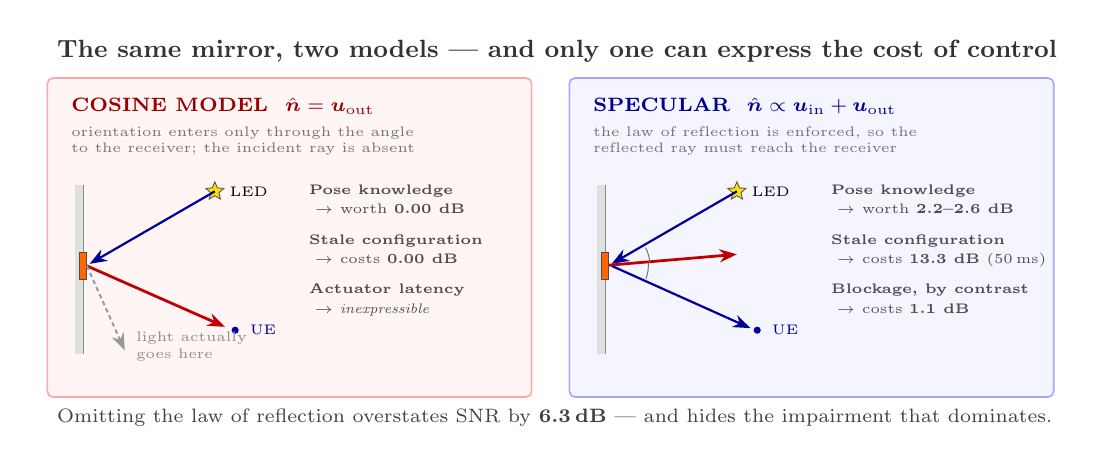
\begin{tikzpicture}[
  >={Stealth[length=2.2mm]},
  font=\footnotesize,
  led/.style={fill=yellow!85!orange, draw=black!70, star, star points=5,
              star point ratio=2.2, inner sep=1.1pt, line width=0.3pt},
  card/.style={rounded corners=2pt, line width=0.6pt},
]

% canvas: 13.28 x 5.31 cm, 2.5:1
\useasboundingbox (0,0) rectangle (13.28,5.31);

%---------------------------------------------------------------- title
\node[anchor=north west, font=\small\bfseries, text=black!80]
  at (0.25,5.28) {The same mirror, two models --- and only one can express
                  the cost of control};

%================================================== LEFT CARD: cosine
\begin{scope}[shift={(0.25,0.62)}]
\draw[card, fill=red!4, draw=red!35] (0,0) rectangle (6.15,4.05);
\node[anchor=north west, font=\scriptsize\bfseries, text=red!60!black]
  at (0.18,3.92) {COSINE MODEL\ \ $\hat{\bm{n}} = \bm{u}_{\mathrm{out}}$};
\node[anchor=north west, font=\tiny, text=black!55, align=left]
  at (0.18,3.56) {orientation enters only through the angle\\
                  to the receiver; the incident ray is absent};

% --- geometry sketch ---
\begin{scope}[shift={(0.45,1.02)}, scale=0.86]
  \draw[black!45, line width=0.6pt] (0,-0.55) -- (0,1.95);
  \fill[black!12] (-0.12,-0.55) rectangle (0,1.95);
  \fill[orange!80!red, draw=black!70, line width=0.3pt]
    (-0.05,0.55) rectangle (0.05,0.95);
  \node[led] at (1.95,1.85) {};
  \fill[blue!65!black] (2.25,-0.20) circle (1.5pt);
  \node[anchor=west, font=\tiny] at (1.95,1.85) {\;LED};
  \node[anchor=west, font=\tiny, text=blue!55!black] at (2.25,-0.20) {\;UE};
  \draw[->, blue!60!black, line width=0.8pt] (1.95,1.85) -- (0.10,0.78);
  \draw[->, red!75!black, line width=1.0pt] (0.06,0.75) -- (2.10,-0.15);
  \draw[->, black!40, line width=0.7pt, dash pattern=on 1.6pt off 1.2pt]
    (0.06,0.75) -- (0.62,-0.50);
  \node[black!45, font=\tiny, anchor=west, align=left, inner sep=1.5pt]
    at (0.72,-0.44) {light actually\\goes here};
\end{scope}

% --- consequences ---
\node[anchor=north west, font=\tiny, text=black!70, align=left]
  at (3.20,2.82)
  {\textbf{Pose knowledge}\\[1pt]
   \hspace*{2pt}$\rightarrow$ worth \textbf{0.00 dB}\\[5pt]
   \textbf{Stale configuration}\\[1pt]
   \hspace*{2pt}$\rightarrow$ costs \textbf{0.00 dB}\\[5pt]
   \textbf{Actuator latency}\\[1pt]
   \hspace*{2pt}$\rightarrow$ \emph{inexpressible}};
\end{scope}

%================================================ RIGHT CARD: specular
\begin{scope}[shift={(6.88,0.62)}]
\draw[card, fill=blue!4, draw=blue!35] (0,0) rectangle (6.15,4.05);
\node[anchor=north west, font=\scriptsize\bfseries, text=blue!55!black]
  at (0.18,3.92)
  {SPECULAR\ \ $\hat{\bm{n}} \propto \bm{u}_{\mathrm{in}}+\bm{u}_{\mathrm{out}}$};
\node[anchor=north west, font=\tiny, text=black!55, align=left]
  at (0.18,3.56) {the law of reflection is enforced, so the\\
                  reflected ray must reach the receiver};

% --- geometry sketch ---
\begin{scope}[shift={(0.45,1.02)}, scale=0.86]
  \draw[black!45, line width=0.6pt] (0,-0.55) -- (0,1.95);
  \fill[black!12] (-0.12,-0.55) rectangle (0,1.95);
  \fill[orange!80!red, draw=black!70, line width=0.3pt]
    (-0.05,0.55) rectangle (0.05,0.95);
  \node[led] at (1.95,1.85) {};
  \fill[blue!65!black] (2.25,-0.20) circle (1.5pt);
  \node[anchor=west, font=\tiny] at (1.95,1.85) {\;LED};
  \node[anchor=west, font=\tiny, text=blue!55!black] at (2.25,-0.20) {\;UE};
  \draw[->, blue!60!black, line width=0.8pt] (1.95,1.85) -- (0.10,0.78);
  \draw[->, blue!60!black, line width=0.8pt] (0.10,0.75) -- (2.15,-0.17);
  \draw[->, red!75!black, line width=1.0pt] (0.06,0.76) -- (1.95,0.92);
  \draw[black!55, line width=0.35pt] (0.60,1.02) arc (28:6:0.58);
  \draw[black!55, line width=0.35pt] (0.64,0.82) arc (6:-20:0.58);
\end{scope}

% --- consequences ---
\node[anchor=north west, font=\tiny, text=black!70, align=left]
  at (3.20,2.82)
  {\textbf{Pose knowledge}\\[1pt]
   \hspace*{2pt}$\rightarrow$ worth \textbf{2.2--2.6 dB}\\[5pt]
   \textbf{Stale configuration}\\[1pt]
   \hspace*{2pt}$\rightarrow$ costs \textbf{13.3 dB} (50\,ms)\\[5pt]
   \textbf{Blockage, by contrast}\\[1pt]
   \hspace*{2pt}$\rightarrow$ costs \textbf{1.1 dB}};
\end{scope}

%---------------------------------------------------------------- footer
\node[anchor=south west, font=\scriptsize, text=black!75]
  at (0.25,0.12)
  {Omitting the law of reflection overstates SNR by \textbf{6.3\,dB} ---
   and hides the impairment that dominates.};

\end{tikzpicture}
\end{document}
